% !TEX root = ../Thesis.tex

\chapter{Theory}

\section{Electron Spin Resonance}
\subsection{Basic Theory}

Electron spin resonance (EPR) functions by detecting the energy difference between the spin states of an electron.
Normally degenerate, the presence of a magnetic field separates the two spin states parallel to it in energy.
The spin state parallel to the magnetic field has a lower energy whilst the anti-parallel state has a higher energy.
For an electron in free space the energy difference is given by:

\begin{equation}
\Delta E = g_e\mu_bB,
\end{equation}

where $g_e$ is the free electron g-factor, $\mu_b$ is the Bohr magneton and $B$ is the magnetic field strength. 
This results in an energy splitting as seen in figure \ref{fig:elecSplit}. 

\begin{figure}
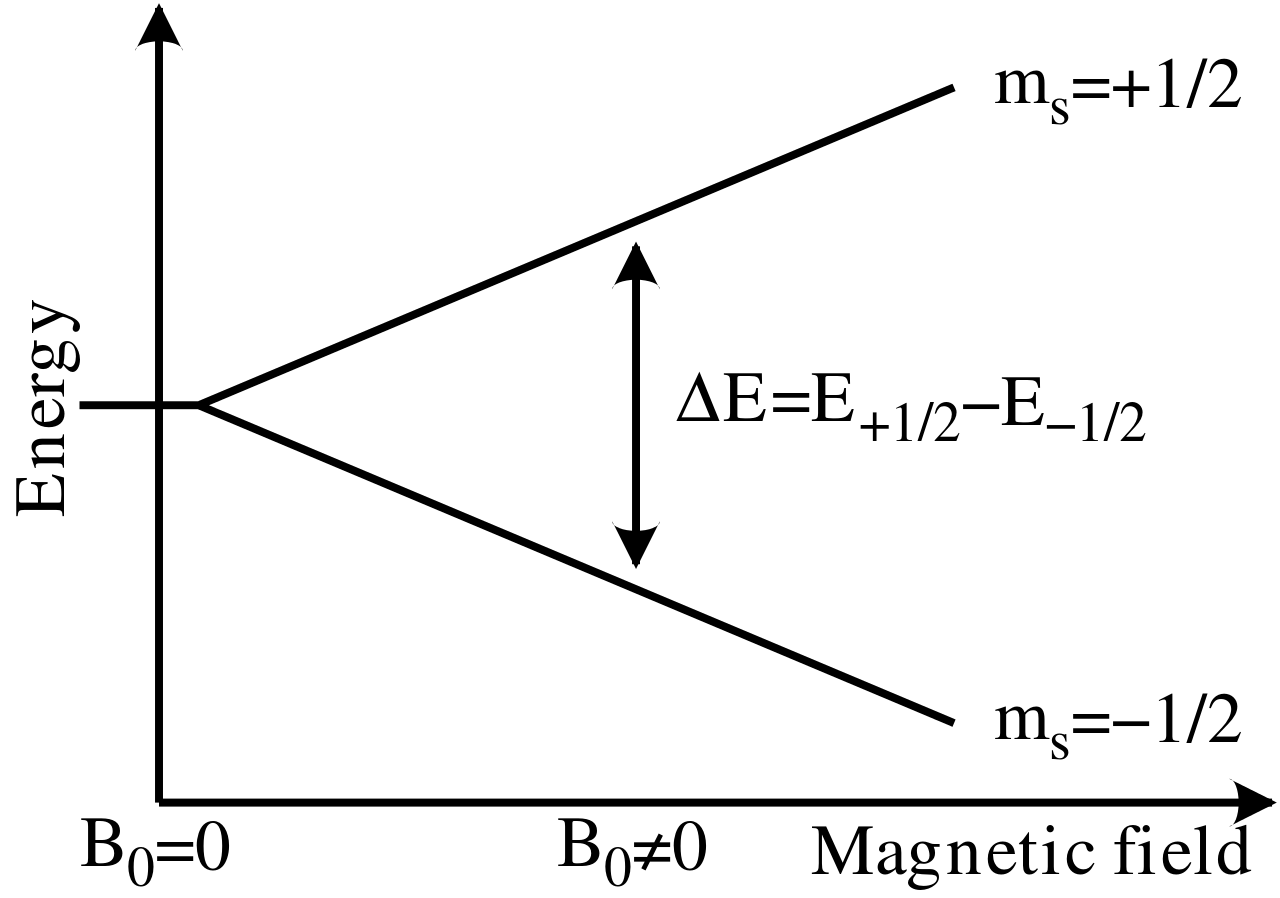
\includegraphics[width = \columnwidth]{Figures/EPR_splitting.png}
\caption[Free electron level splitting]{Spin state energy splitting for a free electron in a magnetic field.}
\label{fig:elecSplit}
\end{figure}

In practice this energy splitting can be detected using continuous wave EPR. Transitions between the spin states will be driven by incident electromagnetic radiation of photon energy equal to the energy gap (i.e $h\nu = g_e\mu_bB$). 
The presence of an EPR transition in a sample can be detected either by applying a constant magnetic field and sweeping EM frequency incident on that sample or vice versa.
In practice, it is the latter that is used for experimental simplicity.
Measuring reflection of radiation from the sample whilst sweeping magnetic field will reveal a drop in reflection at the transition field - when photons are absorbed to drive the spin transition.

\subsection{Pulsed Electron Spin Resonance}